\chapter{Sampling, Waveshaping, und nicht Linearität}
\label{Waveshaping}

\begin{center}
\begin{figure}[h!]
\tikzset{concept/.append style={fill={none}}}
\begin{tikzpicture}
  \path[mindmap,concept color=black,text=black]
    node[concept] {Sampling}
    [clockwise from=0]
    child[concept color=red!50!black] {node[concept] (rec) {recording} }
    child[concept color=green!80!black] {node[concept] (pla) {playback} }
    %   [clockwise from=90]
    %   child { node[concept] {algorithms} }
    %   child { node[concept] {data structures} }
    %   child { node[concept] {pro\-gramming languages} }
    %   child { node[concept] {software engineer\-ing} }
    % }  
    child[concept color=blue] { node[concept] (ram) {in RAM vs. from Disk}[clockwise from=-30]}
    child[concept color=red] { node[concept] (gra) {granular} }
    child[concept color=orange] { node[concept] {Waveshaping and Distortion} };

\begin{pgfonlayer}{background}
	% \draw [draw=green,fill=black, decorate,decoration=circle connection bar]
    \draw [circle connection bar]
    % \path (rec) to[circle connection bar] (pla)
      (rec) edge (pla)
      (gra) edge (pla)
      (ram) edge (pla)
      ;
  \end{pgfonlayer}

\end{tikzpicture}
\caption{Lecture Contents}
\end{figure}
\end{center}

\section{Notizen}

Waveshaping generell.

Evt. Subtraktiver Synth am ende.

Zusammenhang waveshaping, distortion. lookup table, sampling, wavescanning.

Waveshaping = modulation \cite[p.~257]{farnell_designing_2010}

chebyshev

\glqq{}intermod. distortion \grqq{} , vgl. miller puckette, \\
http://msp.ucsd.edu/techniques/latest/book-html/node78.html

middle term! ( (a+b)**2 = a**2 +2ab +b**2 ) 




beispiele:
sinus
vllt:\\
dyn. non-linear functions




\section{Uebersicht}
Zunächst: Sampling, dann lineare transfer function.

\begin{enumerate}
	\item übersicht: fragen wies geht, wie ist es mit Max/MSP?
	\item HÜ ankündigen
	\item neue abstraction: z-1 
	\item Raetsel
	\item Wo letztes mal stehngeblieben? Poly syth fertig?
	\item linearität erklären. Nun Nichtlinearität.
	\item wavetable/lookup wiederholung
	\item Lookup als waveshaping/distortion
	\item waveshaping durch processing vs. durch lookuptable
	\item durchrechnen
	\item chebyshev
	\item Sampling (Ram nicht Ram)
	\item send and receive von GUI f. Hausübung
\end{enumerate}

\section{Waveshaping}
Wikipedia zitat, seite wavesahper:\\
\glqq{}The mathematics of non-linear operations on audio signals is difficult, and not well understood.\grqq{}



\subsection{Einfachster fall, linear transfer function.} % (fold)
\label{sub:linearTrans}

% subsection subsection_name (end)



\begin{figure}[h]
	\begin{center}
		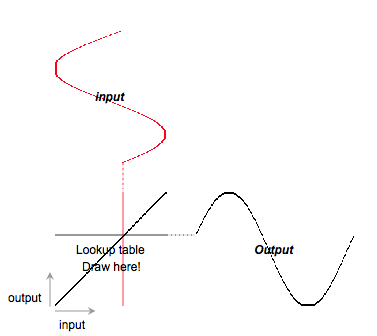
\includegraphics[scale = 1]{img/waveShapingVisual.png}
		\caption{Linear Transfer function}
		\label{fig:linfunct}
	\end{center}
\end{figure}

\subsection{Einfache nicht linearität: \(X ^2\)} % (fold)
\label{sub:nonLinearTrans}

Eine einfacher Fall: ein polynom 2. ordnung soll nun analysiert werden. Die funktion

\begin{equation}
f(x) = x ^ 2
\end{equation}
 wird benutzt.\\

\fbox{
  \parbox{\textwidth}{
    Ein polynom geradzahliger ordnung \(n\) als Transferfunktion produziert immer alle geradzahligen obertöne von \(n\) bis 0, exklusive der grundfrequenz (da ja auch ungerade, 1 ist eine ungerade zahl).\\
Ein polynom ungeradzahliger ordnung \(n\) als Transferfunktion produziert immer alle ungeradzahligen obertöne von \(n\) bis 1, also der grundfrequenz.
  }
}

Wir errechnen was mit einem cosinus signal passiert wenn es durch diese funktion geschickt wird. Also:
\begin{equation}
x = cos(\omega)
\end{equation}
 mit beliebigen omega. (die laufzeit-/index-variable \(t\) bzw. \(n\) wird hier ausgepart, sie ist hier irrelevant).\\
Demnach ist
\begin{equation}
y = cos(\omega)^2
\end{equation}
Das wiederum ergibt
\begin{equation}
y = cos(\omega) \cdot cos(\omega)
\end{equation}
eine simple amplituden modulation eigentlich  \textit{Ringmodulation}. Über Ringmodulation  wiederum wissen wir dass summe und differenz der eingangsfrequenzen ausgegeben werden. Also:
\begin{equation}
y = \frac{cos(\omega+\omega) + cos(\omega-\omega)}{2}
\end{equation}
Also:
\begin{equation}
y = \frac{cos(2 \cdot \omega) + cos(0)}{2} = \frac{cos(2 \cdot \omega )}{2}+\frac{1}{2}
\end{equation}

\textbf{Aber gilt die auch für jeden Input? das würde Bedeuten wir haben einen freq. shifter gebaut? Nein.} Waveshaping ist weit komplexer, was sofort ersichtlich ist wenn man zwei oszillatoren in die funktion schickt:
\begin{equation}
x = cos(\omega_1)+cos(\omega_2) 
\end{equation}
dann
\begin{equation}
y = (cos(\omega_1)+cos(\omega_2) ) ^2
\end{equation}
\begin{equation}
y = cos(\omega_1)^2+cos(\omega_2)^2+2\cdot cos(\omega_1) \cdot cos(\omega_2)
\end{equation}
 
letztendlich kommt man zu:
\begin{equation}
	y = \frac{cos(2 \cdot \omega_1)}{2} + \frac{1}{2} + \frac{cos(2 \cdot \omega_2)}{2} +\frac{1}{2} + 2 \cdot (\frac{cos(\omega_1+\omega_2) + cos(\omega_1-\omega_2)}{2})
\end{equation}



Wieso ist waveshaping praktisch? Amplitudenabhängigkeit d. spectrums. 
Wieso ist waveshaping verwandt mit modulation, sowohl FM, PM als auch AM? Am: siehe \(x^2\). FM: siehe \(f(x)=cos(x)\). Auch kann letztendlich eine transferkuntion in cos/sin bestandteile zerlegt werden um zu einer menge an frequenzmodulationen anzukommen, bzw kann der wavetable als polynom angenähert(o. Taylor entwicklung) werden um bei AM anzukommen.



\section{Sampler}

Sampling von d. Festplatte vs. vom RAM.\\
Zusammen bauen. Geschwindigkeit modulieren etc.\\
Evtl. \texttt{moresampling.pd}, granular sampling kurz erklären.


\begin{figure}[H]
	\begin{center}
		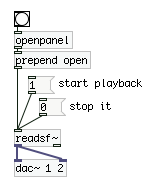
\includegraphics[scale = 1]{img/sampler.png}
		\caption{simpleSampler}
		\label{fig:simpleSampler}
	\end{center}
\end{figure}

\begin{figure}[H]
	\begin{center}
		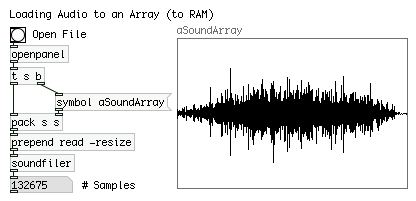
\includegraphics[scale = 1]{img/soundFileToRam.png}
		\caption{sound in Ram}
		\label{fig:soundRam}
	\end{center}
\end{figure}


\begin{figure}[H]
	\begin{center}
		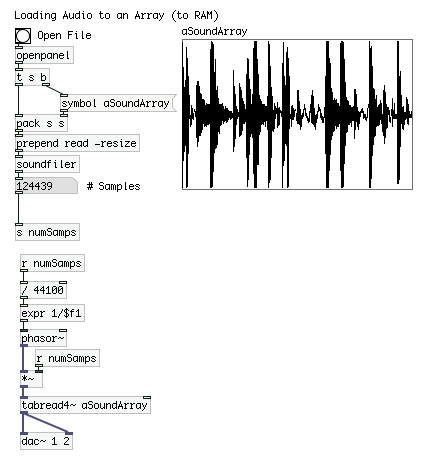
\includegraphics[scale = 1]{img/RamFilePlayback.png}
		\caption{RamFilePlayback}
		\label{fig:RamFilePlayback}
	\end{center}
\end{figure}



\begin{figure}[H]
	\begin{center}
		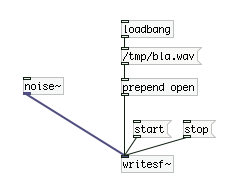
\includegraphics[width = 14cm]{writingAudio.png}
		\caption{writing Audio to disk}
		\label{fig:writing}
	\end{center}
\end{figure}


\begin{figure}[H]
	\begin{center}
		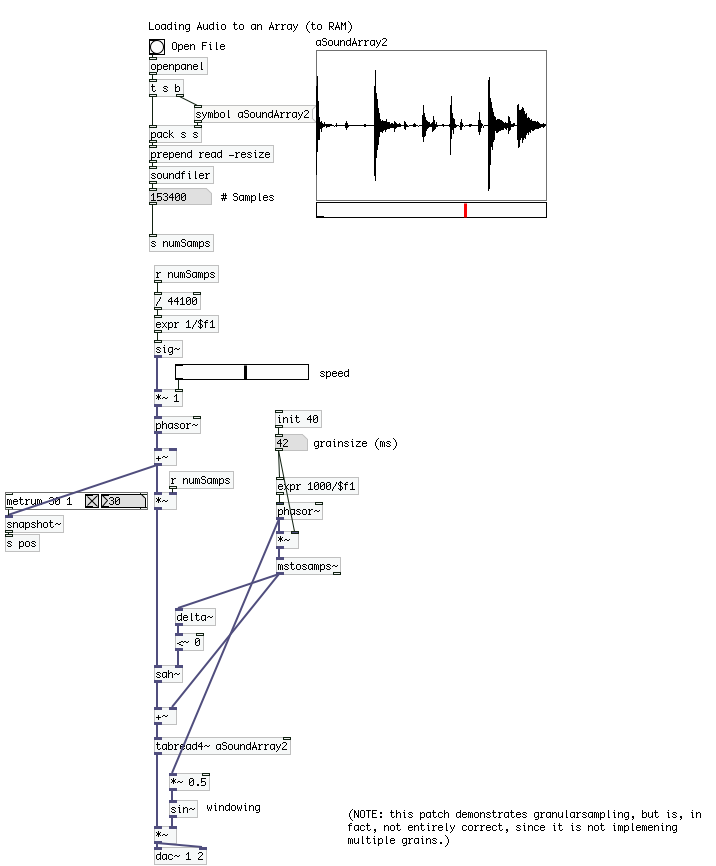
\includegraphics[scale = 0.6]{img/grain.png}
		\caption{moreSamplimg.pd, a simplified version of granular sampling}
		\label{fig:name}
	\end{center}
\end{figure}



\section{Hausübung}
\subsection{Testmodul}

baue ein audio Testmodul mit folgener spezifikation:\\
\begin{itemize}
	\item Ein audio output
	\item verschiedene klangquellen wählbar:
		\begin{enumerate}
			\item White Noise
			\item Sinus (freq. einstellbar)
			\item soundfile (file wählbar)
		\end{enumerate}
	\item GUI
	\item verfügbar(in eurem pfad, und jederzeit abrufbar als abstraction)
	\item output pegel sichtbar (level meter)
\end{itemize}


\begin{figure}[H]
	\begin{center}
		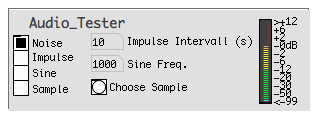
\includegraphics[scale = 1]{img/audioTester.png}
		\caption{audioTester.pd, zu bauen als Hausübung}
		\label{fig:audiotester}
	\end{center}
\end{figure}

\subsection{Distortion}
Baue eine besonders wohlklingende Distortion, inkl. User interface.

